%%
%% This is file `sample-sigconf.tex',
%% generated with the docstrip utility.
%%
%% The original source files were:
%%
%% samples.dtx  (with options: `sigconf')
%% 
%% IMPORTANT NOTICE:
%% 
%% For the copyright see the source file.
%% 
%% Any modified versions of this file must be renamed
%% with new filenames distinct from sample-sigconf.tex.
%% 
%% For distribution of the original source see the terms
%% for copying and modification in the file samples.dtx.
%% 
%% This generated file may be distributed as long as the
%% original source files, as listed above, are part of the
%% same distribution. (The sources need not necessarily be
%% in the same archive or directory.)
%%
%%
%% Commands for TeXCount
%TC:macro \cite [option:text,text]
%TC:macro \citep [option:text,text]
%TC:macro \citet [option:text,text]
%TC:envir table 0 1
%TC:envir table* 0 1
%TC:envir tabular [ignore] word
%TC:envir displaymath 0 word
%TC:envir math 0 word
%TC:envir comment 0 0
%%
%%
%% The first command in your LaTeX source must be the \documentclass command.
\documentclass[sigconf]{acmart}
\usepackage{balance} % For balanced columns on the last page
\usepackage[binary-units]{siunitx}
\usepackage{listings}

\sisetup{separate-uncertainty=true}

% Visible TODO notes
\newcommand{\todo}[1]{\textbf{\textsc{\textcolor{red}{(TODO: #1)}}}}

% Code colouring
\definecolor{NavyBlue}{rgb}{0.0,0.0,0.5}
\definecolor{OliveGreen}{rgb}{0.5,0.5,0.0}
\definecolor{Mulberry}{rgb}{0.77,0.29,0.55}
\definecolor{Maroon}{rgb}{0.5,0.0,0.0}
\lstset{language=Python,morekeywords={True,False},showstringspaces=false,basicstyle=\small\ttfamily\bfseries,keywordstyle=\color{Mulberry}\bfseries,identifierstyle=\color{NavyBlue}\bfseries,stringstyle=\ttfamily\color{OliveGreen}\bfseries,commentstyle=\ttfamily\color{Maroon}\bfseries,frame=single,upquote=true,morekeywords={True,False}}


%%
%% \BibTeX command to typeset BibTeX logo in the docs
\AtBeginDocument{%
  \providecommand\BibTeX{{%
    \normalfont B\kern-0.5em{\scshape i\kern-0.25em b}\kern-0.8em\TeX}}}

%% Rights management information.  This information is sent to you
%% when you complete the rights form.  These commands have SAMPLE
%% values in them; it is your responsibility as an author to replace
%% the commands and values with those provided to you when you
%% complete the rights form.
\copyrightyear{2022}
\acmYear{2022}
\setcopyright{rightsretained}
\acmConference[NICE 2023]{Neuro-Inspired Computational Elements Conference}{April 11-April 14, 2023}{San Antonio, USA}
\acmBooktitle{Neuro-Inspired Computational Elements Conference (NICE 2023), April 11-April 14, 2023, San Antonio, USA}
\acmDOI{XXXXXXX.XXXXXXX}
\acmISBN{978-1-4503-XXXX-X/18/06}


%%
%% Submission ID.
%% Use this when submitting an article to a sponsored event. You'll
%% receive a unique submission ID from the organizers
%% of the event, and this ID should be used as the parameter to this command.
%%\acmSubmissionID{123-A56-BU3}

%%
%% The majority of ACM publications use numbered citations and
%% references.  The command \citestyle{authoryear} switches to the
%% "author year" style.
%%
%% If you are preparing content for an event
%% sponsored by ACM SIGGRAPH, you must use the "author year" style of
%% citations and references.
%% Uncommenting
%% the next command will enable that style.
%%\citestyle{acmauthoryear}

%%
%% end of the preamble, start of the body of the document source.
\begin{document}

%%maintanance
%% The "title" command has an optional parameter,
%% allowing the author to define a "short title" to be used in page headers.
\title{mlGeNN: user-friendly and efficient spike-based Machine Learning}

%%
%% The "author" command and its associated commands are used to define
%% the authors and their affiliations.
%% Of note is the shared affiliation of the first two authors, and the
%% "authornote" and "authornotemark" commands
%% used to denote shared contribution to the research.
\author{James C Knight}
\email{J.C.Knight@sussex.ac.uk}
\orcid{0000-0003-0577-0074}
\affiliation{%
  \institution{University of Sussex}
  \department{School of Engineering and Informatics}
  \city{Brighton}
  \country{United Kingdom}
}

\author{Thomas Nowotny}
\email{T.Nowotny@sussex.ac.uk}
\orcid{0000-0002-4451-915X}
\affiliation{%
  \institution{University of Sussex}
  \department{School of Engineering and Informatics}
  \city{Brighton}
  \country{United Kingdom}
}
%%
%% By default, the full list of authors will be used in the page
%% headers. Often, this list is too long, and will overlap
%% other information printed in the page headers. This command allows
%% the author to define a more concise list
%% of authors' names for this purpose.
\renewcommand{\shortauthors}{Knight and Nowotny}

%%
%% The abstract is a short summary of the work to be presented in the
%% article.
\begin{abstract}
    To demonstrate the value of mlGeNN in this space, we present the results of an exploration of shallow classifier architectures for the classification of the DVS gesture dataset. 
\end{abstract}

%%
%% The code below is generated by the tool at http://dl.acm.org/ccs.cfm.
%% Please copy and paste the code instead of the example below.
%%
\begin{CCSXML}
<ccs2012>
   <concept>
       <concept_id>10010147.10010257.10010293.10011809</concept_id>
       <concept_desc>Computing methodologies~Bio-inspired approaches</concept_desc>
       <concept_significance>300</concept_significance>
       </concept>
   <concept>
       <concept_id>10010147.10010257.10010258.10010259</concept_id>
       <concept_desc>Computing meis thodologies~Supervised learning</concept_desc>
       <concept_significance>300</concept_significance>
       </concept>
   <concept>
       <concept_id>10010147.10010169.10010170.10010173</concept_id>
       <concept_desc>Computing methodologies~Vector / streaming algorithms</concept_desc>
       <concept_significance>300</concept_significance>
       </concept>
 </ccs2012>
\end{CCSXML}

\ccsdesc[300]{Computing methodologies~Bio-inspired approaches}
\ccsdesc[300]{Computing methodologies~Supervised learning}
\ccsdesc[300]{Computing methodologies~Vector / streaming algorithms}

%%is 
%% Keywords. The author(s) should pick words that accurately describe
%% the work being presented. Separate the keywords with commas.
\keywords{spiking neural networks, efficient simulation, GPU}

%%
%% This command processes the author and affiliation and title
%% information and builds the first part of the formatted document.
\maketitle

\section{Introduction}
The development of efficient SNN simulators has been a key area of computational neuroscience research for several decades~\citep{carnevale2006neuron, Gewaltig2007, Golosio2021, Akar2019,Yavuz2016}.
However, these simulators are not well-suited to the types of model and the workflows required for spike-based machine learning research.
As such, many ML researchers have chosen to build libraries~\citep{norse2021, SpikingJelly, eshraghian2021training,Hazan2018}\todo{cite neko} on top of frameworks like PyTorch which allow SNNs to be defined in a familiar environment for ML researchers,.
When using these libraries, the activity of a population of neurons is typically represented as a vector of activations and, for an SNN, this vector is populated with ones for spiking and zeros for non-spiking neurons. 
This representation allows one to apply the existing infrastructure of the underlying ML library to SNNs but, as real neurons often spike at comparatively low rates, propagating the activity of inactive neurons through the network leads to unnecessary computation.
Additionally, the connections between populations of real neurons are sparse which, using a standard ML library, would typically be implemented as a weight matrix containing many zeros.

Both choices are inefficient so, we have developed mlGeNN -- a new library for spike-based ML built on the GPU-optimised sparse data structures and algorithms provided by our GeNN simulator~\todo{cite ourselves!}.
We previously presented an initial version of mlGeNN~\todo{cite} which provided workflows for converting ANNs trained using TensorFlow~\todo{cite} into SNNs for simulation using GeNN.
However, while we found that performing inference using our converted SNNs was faster than competing libraries, SNNs are inherantly at a disadvantage for static image classification as by their nature they turn what an ANN library could perform in a single inference step into something that needs simulating for several timesteps.

\section{mlGeNN}
\subsection{Describing models}
\begin{itemize}
    \item functional vs sequential abstractions -> connection based and sequential
    \item Abstraction - synapses/feedback connections vs compilers
\end{itemize}

Synaptic connectivity in the brain is structured but highly recurrent and this makes the underlying Directed Acyclical Graphs~(DAG) model used by typical deep learning libraries a poor fit as

One of the key aims of mlGeNN is to make it simple to define Spiking Neural Networks (SNNs) with arbitrary topologys that are awk. 
Networks consist of homogenous groups of neurons described by \lstinline{Population} objects connected together with \lstinline{Connection} objects.
All populations and connections are owned by a \lstinline{Network} which acts as a context manager so a network with two populations of neurons could be simply created like:

\begin{lstlisting}[language=Python]
from ml_genn import (Connection, Population,
                     Network)

network = Network()
with network:
    a = Population("poisson_input", 100)
    b = Population("integrate_fire", 100,
                   readout="spike_count")

    Connection(a, b, Dense(1.0))
\end{lstlisting}

For simplicity, in this example, built in neuron models with default parameters are specified using strings.
However, if you wish to override some of the default model parameters, use a model that does not have default parameters or use a model not built into mlGeNN, you can also specify a neuron model using a \lstinline{Neuron} class instance.
For example, if we wished for the poisson population to emit positive and negative spikes for positive and negative input values and for the integrate-and-fire 
neuron to have a higher firing threshold we could instantiate \lstinline{PoissonInput} and \lstinline{IntegrateFire} objects ourselves like:

\begin{lstlisting}[language=Python]
from ml_genn import (Connection, Population,
                     Network)
from ml_genn.neurons import (PoissonInput,
                             IntegrateFire)

network = Network()
with network:
    a = Population(
        PoissonInput(signed_spikes=True), 100)
    b = Population(
        IntegrateFire(v_thresh=2.0), 100,
        readout="spike_count")

    Connection(a, b, Dense(1.0))
\end{lstlisting}

By default, \lstinline{Connection} objects use a `delta' synapse model where the accumulated weight of incoming spikes is directly injected into neurons. 
However, if you wish to use a somewhat more realistic model where inputs are \emph{shaped} to mimic the dynamics of real ion channels, this can be swapped
This same general principle is also used for configuring many other aspects of mlGeNN, including loss functions, metrics and readouts. 

While the flexibility to create networks with any topology is very useful, mlGeNN also provides a \lstinline{SequentialNetwork} wrapper class -- inspired by \lstinline{Sequential} models in Keras -- for specifying common feedforward model more tersely:

\begin{lstlisting}[language=Python]
from ml_genn import (InputLayer, Layer,
                     SequentialNetwork)

network = SequentialNetwork()
with network:
    a = InputLayer("poisson_input", 100)
    b = Layer(Dense(1.0), "integrate_fire", 100,
              readout="spike_count")
\end{lstlisting}

Finally, in the same way that Keras can easily be extended by subclassing built in classes and implementing new functionality using TensorFlow constructs, mlGeNN can be extended by subclassing  built in classes and providing PyGeNN model descriptions. 
A full description of the model description syntax is beyond the scope of this work but, is described in more detail in our documentation~\todo{cite} and previous work~\todo{cite pygenn}.
Nonetheless, the following example illustrates how a minimal Integrate-and-Fire neuron model could be defined for use in mlGeNN:

\begin{lstlisting}[language=Python]
from ml_genn.neuron import Neuron
from ml_genn.utils.model import NeuronModel
from ml_genn.utils.value import ValueDescriptor

genn_model = {
    "var_name_types": [("V", "scalar")],
    "sim_code": "$(V) += $(Isyn);",
    "threshold_condition_code": "$(V) >= 1.0",
    "reset_code": "$(V) = 0.0;",
    "is_auto_refractory_required": False}

class IntegrateFire(Neuron):
    v = ValueDescriptor("V")

    def __init__(self, v = 0.0, softmax = False, 
                 readout=None):
        super(IntegrateFire, self).__init__(
            softmax, readout)
        self.v = v

    def get_model(self, population, dt):
        return NeuronModel.from_val_descriptors(
            genn_model, "V", self, dt)
\end{lstlisting}



\subsection{Compiling and using models}
Once a network structure has been defined using the functionality described in the previous section, mlGeNN provides a range of \emph{compilers} to produce GeNN models which can be used for training or inference.
The simplest compiler is the \lstinline{InferenceCompiler} which builds a GeNN model with static weights and parallel batching support for efficiently performing inference on an SNN model:

\begin{lstlisting}[language=Python]
compiler = InferenceCompiler(
    evaluate_timesteps=1500, batch_size=512)

compiled_net = compiler.compile(network)
\end{lstlisting}

The resulting \lstinline{compiled_net} object can then be used to evaluate the network on a dataset:

\begin{lstlisting}[language=Python]
metrics, _  = compiled_net.evaluate({input: spikes},
                                    {output: labels})
\end{lstlisting}

By default, the evaluation method calculates sparse categorical accuracy against the labels but mlGeNN provides alternative metrics for regression tasks and custom metrics can be easily implemented.

\todo{talk a little about eProp}
\begin{lstlisting}[language=Python]
compiler = EPropCompiler(
    example_timesteps=1500,
    losses="sparse_categorical_crossentropy",
    optimiser="adam", batch_size=512)

compiled_net = compiler.compile(network)
\end{lstlisting}

\todo{talk a little about callbacks etc for recording etc}

\section{Results}
In order to demonstrate the value of mlGeNN for spike-based ML research, here we present the results of a small exploration of SNN architectures, trained using e-prop~\todo{cite maas} on the DVS gesture dataset which has been recently used to evaluate the EGRU~\todo{cite} and FPTT~\todo{cite} learning rules.
This dataset was provided by the Tonic library~\todo{cite} and, while mlGeNN does not depend on this library, it includes a \lstinline{preprocess_tonic_spikes} helper function which converts spike trains from Tonic datasets into mlGeNN's internal format.

\begin{figure*}[t]
  \centering
  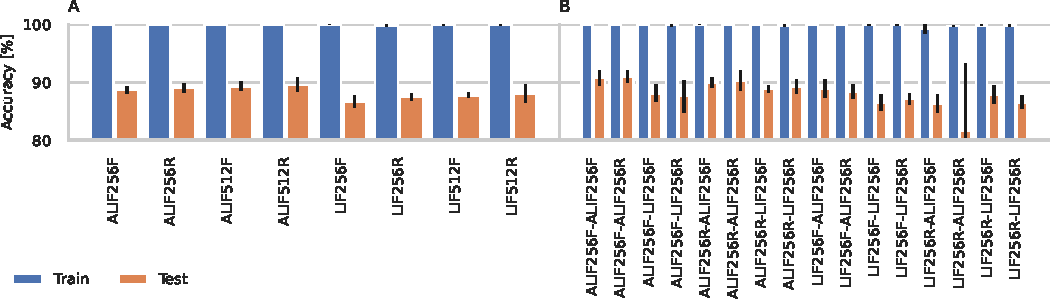
\includegraphics{figures/dense_accuracy.pdf}
  \caption{Accuracy on the testing and training set of the DVS gesture dataset~\todo{cite} on one (A) and two (B) layer eProp classifiers.
  All models were trained for 100 epochs with a batch size of 512.
  \todo{finish training 1024 neuron models}
  \todo{investigate gaps}
  Bars signify the mean and error bars the standard deviation of 5 models trained with different seeds.}
  \label{fig:dense_accuracy}
\end{figure*}

\subsection{Accuracy}
Figure~\ref{fig:dense_accuracy} shows the accuracy of a wide selection of one and two layer classifier models trained with e-prop.
These include configurations with and without recurrent connections and using both Adaptive and standard Leaky Integrate-and-Fire~(LIF and ALIF) neuron models.
Of the single layer classifiers, the variant with a single layer of 512 recurrently connected ALIF neurons performs the best, achieving a mean accuracy of \SI{89.39}{\percent} on the test set.
Although this model only has a single hidden layer and around \num{1.3E6} parameters, it out-performs a two layer EGRU model~\todo{cite} with over $4\times$ as many parameters which achieved \SI{88.02}{\percent} accuracy.
\begin{itemize}
    \item FPTT shallow recurrent \SI{91.89 \pm 0.16}{\percent} 512 neuron encoder for each channel, feeding into recurrent population of 512 neurons
    \item EGRU two EGRU layers of 512 \SI{88.02}{\percent} (5.5M parameters), two EGRU layers of 1024 \SI{90.22}{\percent} (15.75M parameters)
    \item Take best architecture and explore sparsity
\end{itemize}

\subsection{Performance}
\begin{itemize}
    \item Training time - compare to FPTT \SI{400}{\milli\second} per frame with batch size 64 on some sort of \SI{24}{\giga\byte} GPU
    \item Inference time CPU and GPU - compare to real-time
    \item Show effect of sparsity on performance
\end{itemize}

\section{Conclusions}
The results we have presented in this paper demonstrate that the approximation used by the e-prop learning rule do not necessarily prevent it enablig competitive performane in relatively complex datasets, e-prop does have some significant issues.
\begin{itemize}
    \item Eligibility traces are unique to each pair of connected pre and postsynaptic neurons so cannot be efficiently added to convolutional models
    \item The e-prop learning rule requires time-driven updates which dominate the time taken to \emph{train} these models although, by using sparse connectivity, this 
\end{itemize}
However, 
Therefore, we are working to implement the fully event-driven EventProp~\citep{Wunderlich2021} learning rule in GeNN which will allow training times to also benefit from temporal sparsity.
Finally, the models presented in this paper are all densely connected so are not taking advantage of connection sparsity.
We are working in parallel to address this by combining these learning rules with the Deep-R~\citep{Bellec2018a} rewiring rule, enabling SNN classifiers to take advantage of GeNN's support for efficient sparse connectivity~\citep{Knight2018}.


%%
%% The acknowledgments section is defined using the "acks" environment
%% (and NOT an unnumbered section). This ensures the proper
%% identification of the section in the article metadata, and the
%% consistent spelling of the heading.
\begin{acks}
This work was funded by the EPSRC (grant numbers EP/V052241/1 and EP/S030964/1) and the EU's Horizon 2020 program (grant agreement 945539).
Compute time was provided through Gauss Centre for Supercomputing application number 21018 and EPSRC (grant number EP/T022205/1).
\end{acks}

%%
%% The next two lines define the bibliography style to be used, and
%% the bibliography file.
\balance
\bibliographystyle{ACM-Reference-Format}
\bibliography{ml_genn_eprop}

\end{document}
\endinput
%%
%% End of file `sample-sigconf.tex'.
